\chapter{The Kalman filter}
\label{ch:kalman}

If the motion and sensor models are linear and every noise is Gaussian,
the Bayes filter has an exact, closed-form solution: a Gaussian belief
stays Gaussian, and only its mean and covariance need to be carried
forward. That solution is the Kalman filter. This chapter derives it from
two facts about Gaussians, applies it to a robot made linear by a compass,
and introduces the tool used throughout the rest of the book to decide
whether a filter is \emph{honest}: the NEES test.

\section{Two facts about Gaussians}

The Bayes filter does two things to a belief: it pushes it through the
motion model, and it conditions it on a measurement. For Gaussians both
operations have closed forms. A linear map of a Gaussian is Gaussian
(\cref{lem:affine}), and a Gaussian conditioned on a linear measurement is
Gaussian (\cref{thm:conditioning}). The Kalman filter is these two facts
applied in turn.

Notation: for random vectors $X$ and $Y$ with means $\bmu_x$ and $\bmu_y$,
$\Cov(X,Y)=\E[(X-\bmu_x)(Y-\bmu_y)\T]$ is their \emph{cross-covariance}
matrix, and $\Cov(X)=\Cov(X,X)$. For matrices $A$ and $B$,
\[
  \Cov(AX,BY)=\E\bigl[A(X-\bmu_x)(Y-\bmu_y)\T B\T\bigr]
  =A\,\E\bigl[(X-\bmu_x)(Y-\bmu_y)\T\bigr]\,B\T=A\Cov(X,Y)B\T,
\]
because $AX$ has the mean $A\bmu_x$, $(B(Y-\bmu_y))\T=(Y-\bmu_y)\T B\T$,
and constant matrices come out of an expectation. Two vectors are \emph{uncorrelated} if
$\Cov(X,Y)=0$. A symmetric matrix $\Sigma$ is \emph{positive
semi-definite}, written $\Sigma\succeq0$, if
$\vect a\T\Sigma\vect a\ge0$ for every vector $\vect a$, and
\emph{positive definite}, $\Sigma\succ0$, if moreover
$\vect a\T\Sigma\vect a>0$ for every $\vect a\neq\vect0$. Every covariance
matrix is positive semi-definite, because $\vect a\T\Cov(X)\,\vect a$ is
the variance of the number $\vect a\T X$. It is positive definite when no
combination of the coordinates of $X$ is known exactly. Finally, two
vectors $X$ and $Y$ are called \emph{jointly Gaussian} when the vector
$(X,Y)$ obtained by stacking them is Gaussian in the sense of the next
definition.

\begin{definition}{Multivariate Gaussian}{gaussian}
A random vector $X\in\R^n$ is Gaussian, $X\sim\Normal(\bmu,\Sigma)$ with
$\Sigma$ symmetric positive semi-definite, if every linear combination
$\vect{a}\T X$ is a Gaussian (possibly with variance zero, that is, a
constant) with mean
$\vect{a}\T\bmu$ and variance $\vect{a}\T\Sigma\vect{a}$.
\end{definition}

When $\Sigma$ is positive definite, such a vector has the density
\begin{equation}\label{eq:gaussdensity}
  \Normal(\x;\bmu,\Sigma)=\det(2\pi\Sigma)^{-1/2}
  \exp\bigl(-\tfrac12(\x-\bmu)\T\Sigma^{-1}(\x-\bmu)\bigr).
\end{equation}
This is a consequence of the definition, proved in \cref{lem:dichotomy}.

The level sets of this density are ellipsoids centred at $\bmu$
(ellipses in the plane, \cref{fig:gaussian}, left). Their axes point along
the eigenvectors of $\Sigma$, and the half-length of each axis is
proportional to the standard deviation in its direction, the square root
of the eigenvalue. The figures of this book draw a planar Gaussian as its
``$2\sigma$ ellipse'', the level set whose half-axes are twice these
standard deviations; it contains $86\%$ of the probability. Here is
why. Write $X=\bmu+L\vect g$ with $LL\T=\Sigma$, as in the proof of
\cref{lem:dichotomy} below: $\vect g$ is a pair of independent standard
normals, with the density $e^{-\norm{\vect g}^2/2}/(2\pi)$, and the
$2\sigma$ ellipse is the image of the disc $\norm{\vect g}\le2$. In polar
coordinates $(r,\alpha)$, the area element is $r\,\mathrm dr\,\mathrm
d\alpha$, and the disc of radius $\rho$ has the probability
\[
  \int_0^{2\pi}\!\!\int_0^\rho\frac{e^{-r^2/2}}{2\pi}\,r\,\mathrm dr\,
  \mathrm d\alpha
  =\underbrace{\frac{1}{2\pi}\int_0^{2\pi}\mathrm d\alpha}_{=1}\;
   \Bigl[-e^{-r^2/2}\Bigr]_0^\rho
  =1-e^{-\rho^2/2},
\]
since $-e^{-r^2/2}$ has the derivative $r\,e^{-r^2/2}$. Equivalently,
with $x=\rho^2$,
\begin{equation}\label{eq:chi2tail}
  \Pr\bigl(\norm{\vect g}^2>x\bigr)=e^{-x/2}\qquad(x\ge0),
\end{equation}
and for $\rho=2$ the disc has the probability $1-e^{-2}\approx0.86$.

\emph{Characteristic functions.} Two proofs below use the
\emph{characteristic function} of a random vector $X$, the function
$\vect a\mapsto\E[e^{\ii\vect a\T X}]$, where $\ii^2=-1$, and two facts
about it.
\begin{itemize}[nosep]
  \item A distribution is determined by its characteristic function: two
        random vectors with the same characteristic function have the
        same distribution (the uniqueness theorem of probability; see
        Billingsley in the references).
  \item For a scalar Gaussian $G$ with mean $m$ and variance $v$, and a
        number $u$, $\E[e^{\ii uG}]=e^{\ii um-u^2v/2}$. For $m=0$ and
        $v=1$ this is computed in \cref{sec:feyn-complex}; in general
        $uG=um+u\sqrt v\,G_0$ with $G_0$ standard, which gives the factor
        $e^{\ii um}$ and replaces $u^2$ by $u^2v$.
\end{itemize}

\begin{lemma}{Affine maps and sums}{affine}
If $X\sim\Normal(\bmu,\Sigma)$, then $AX+\vect{b}\sim\Normal(A\bmu+\vect{b},
A\Sigma A\T)$. If moreover $W\sim\Normal(\vect0,Q)$ is independent of
$X$, then $AX+\vect{b}+W\sim\Normal(A\bmu+\vect{b},A\Sigma A\T+Q)$.
\end{lemma}

\begin{proof}
\emph{The affine map.} By \cref{def:gaussian}, we must show that every
combination $\vect a\T(AX+\vect b)$ is Gaussian with the right mean and
variance. It equals $(A\T\vect a)\T X+\vect a\T\vect b$: the combination
of $X$ with the vector $A\T\vect a$, which is Gaussian with mean
$(A\T\vect a)\T\bmu=\vect a\T A\bmu$ and variance $(A\T\vect a)\T\Sigma
(A\T\vect a)=\vect a\T A\Sigma A\T\vect a$, plus the constant
$\vect a\T\vect b$. So it is Gaussian with mean $\vect a\T(A\bmu+\vect b)$
and variance $\vect a\T(A\Sigma A\T)\vect a$, as $\Normal(A\bmu+\vect b,
A\Sigma A\T)$ requires.

\emph{The pair $(X,W)$ is Gaussian.} Take a combination $\vect a\T X+\vect
c\T W$. Its two terms $G_1=\vect a\T X$ and $G_2=\vect c\T W$ are
independent scalar Gaussians, with means $m_1=\vect a\T\bmu$, $m_2=0$ and
variances $v_1=\vect a\T\Sigma\vect a$, $v_2=\vect c\T Q\vect c$. For
every number $u$,
\[
  \E\bigl[e^{\ii u(G_1+G_2)}\bigr]
  =\E\bigl[e^{\ii uG_1}\bigr]\,\E\bigl[e^{\ii uG_2}\bigr]
  =e^{\ii um_1-u^2v_1/2}\,e^{\ii um_2-u^2v_2/2}
  =e^{\ii u(m_1+m_2)-u^2(v_1+v_2)/2},
\]
by independence, then by the characteristic function of a scalar
Gaussian. This is the characteristic function of
$\Normal(m_1+m_2,v_1+v_2)$, so, by uniqueness, $G_1+G_2$ is that
Gaussian. Hence $(X,W)$ is Gaussian, with the mean $(\bmu,\vect0)$ and the
covariance $\begin{psmallmatrix}\Sigma&0\\0&Q\end{psmallmatrix}$: the
off-diagonal blocks are $\Cov(X,W)=0$ because $X$ and $W$ are
independent.

\emph{The sum.} $AX+\vect b+W=[A\ \,I]\begin{psmallmatrix}X\\W
\end{psmallmatrix}+\vect b$ is an affine map of the Gaussian pair. By the
first part, it is Gaussian with the mean $A\bmu+\vect b$ and the covariance
\[
  [A\ \,I]\begin{pmatrix}\Sigma&0\\0&Q\end{pmatrix}
  \begin{pmatrix}A\T\\I\end{pmatrix}=A\Sigma A\T+Q .
\]
\end{proof}

Independent random vectors are always uncorrelated. For jointly Gaussian
vectors the converse holds, a fact used several times below.

\begin{lemma}{Uncorrelated jointly Gaussian vectors are independent}{uncorr}
If $(X,Y)$ is jointly Gaussian and $\Cov(X,Y)=0$, then $X$ and $Y$ are
independent.
\end{lemma}

\begin{proof}
Write $\Sigma_{xx}=\Cov(X)$ and $\Sigma_{yy}=\Cov(Y)$. For any $\vect a,\vect
b$, the scalar $\vect a\T X+\vect b\T Y$ is Gaussian, because $(X,Y)$ is
jointly Gaussian. Its mean is $\vect a\T\bmu_x+\vect b\T\bmu_y$, and its
variance is
\[
  \Var(\vect a\T X+\vect b\T Y)
  =\vect a\T\Sigma_{xx}\vect a+2\,\vect a\T\Cov(X,Y)\,\vect b
   +\vect b\T\Sigma_{yy}\vect b
  =\vect a\T\Sigma_{xx}\vect a+\vect b\T\Sigma_{yy}\vect b ,
\]
the cross term being zero. With the characteristic function of a scalar
Gaussian (above, with $u=1$), this gives
\[
  \E\bigl[e^{\ii(\vect a\T X+\vect b\T Y)}\bigr]
  =e^{\ii\vect a\T\bmu_x-\frac12\vect a\T\Sigma_{xx}\vect a}\;
   e^{\ii\vect b\T\bmu_y-\frac12\vect b\T\Sigma_{yy}\vect b}
  =\E\bigl[e^{\ii\vect a\T X}\bigr]\,\E\bigl[e^{\ii\vect b\T Y}\bigr].
\]
The joint characteristic function is the product of the two marginal
ones. Now take $X'$ and $Y'$ \emph{independent}, with the distributions of
$X$ and $Y$: by independence their joint characteristic function is the
same product. By uniqueness, $(X,Y)$ has the distribution of $(X',Y')$,
so $X$ and $Y$ are independent.
\end{proof}

The definition allows a covariance $\Sigma$ that is not invertible. The
next lemma says what such a Gaussian looks like; it is not needed to
derive the Kalman filter, but \cref{prop:degenerate} relies on it.

\begin{lemma}{A Gaussian has a density or lies in a subspace}{dichotomy}
Let $X\sim\Normal(\bmu,\Sigma)$ in $\R^n$.
\begin{enumerate}[label=(\roman*),nosep]
\item If $\Sigma$ is invertible, $X$ has the density
  \eqref{eq:gaussdensity}.
\item If $\Sigma$ is singular, then with probability one $X$ lies in the
  affine subspace $\bmu+\operatorname{range}(\Sigma)$, of dimension
  $\operatorname{rank}(\Sigma)<n$, and $X$ has no density on $\R^n$.
\end{enumerate}
\end{lemma}

\begin{proof}
(i) $\Sigma$ is positive definite, so $\Sigma=LL\T$ with $L$ invertible
(Cholesky). Let $Z=L^{-1}(X-\bmu)$. By \cref{lem:affine}, $Z$ is Gaussian
with mean $\vect0$ and covariance $L^{-1}\Sigma L^{-\mathsf T}=I$. Its
components are jointly Gaussian and uncorrelated, hence independent
standard normals (apply \cref{lem:uncorr} to the first component against
the others, then to the second against the remaining ones, and so on), so $Z$ has the density
$(2\pi)^{-n/2}\exp(-\tfrac12\norm{\vect z}^2)$. Since $X=\bmu+LZ$ is an invertible affine map of $Z$, the
change-of-variables formula says that the density of $X$ at $\x$ is the
density of $Z$ at the point $L^{-1}(\x-\bmu)$ that is mapped to $\x$,
divided by $\lvert\det L\rvert$, the factor by which $L$ multiplies
volumes:
\[
  p_X(\x)=\frac{(2\pi)^{-n/2}}{\lvert\det L\rvert}
  \exp\bigl(-\tfrac12\norm{L^{-1}(\x-\bmu)}^2\bigr).
\]
This is the density \eqref{eq:gaussdensity}. First,
$\det\Sigma=\det L\,\det L\T=(\det L)^2$, so $\lvert\det L\rvert
=\sqrt{\det\Sigma}$, and $(2\pi)^{-n/2}(\det\Sigma)^{-1/2}
=\det(2\pi\Sigma)^{-1/2}$ because $\det(2\pi\Sigma)=(2\pi)^n\det\Sigma$.
Second, $\norm{L^{-1}(\x-\bmu)}^2=(\x-\bmu)\T L^{-\mathsf T}L^{-1}(\x-\bmu)
=(\x-\bmu)\T(LL\T)^{-1}(\x-\bmu)=(\x-\bmu)\T\Sigma^{-1}(\x-\bmu)$.

(ii) Take $\vect n\neq\vect0$ with $\Sigma\vect n=\vect0$. The scalar
$\vect n\T X$ has variance $\vect n\T\Sigma\vect n=0$, and a random
variable with zero variance equals its mean with probability one:
$\vect n\T(X-\bmu)=0$. So $X$ lies in the hyperplane through $\bmu$
perpendicular to $\vect n$. Applying this to a basis
$\vect n_1,\dots,\vect n_k$ of the null space of $\Sigma$, $X-\bmu$ is,
with probability one, orthogonal to the whole null space. For a symmetric
matrix the orthogonal complement of the null space is the range, so
$X\in\bmu+\operatorname{range}(\Sigma)$, a subspace of dimension
$n-k=\operatorname{rank}(\Sigma)$. A proper affine subspace has zero
volume, and a distribution with a density gives probability zero to every
set of zero volume: $X$ has no density.
\end{proof}

Part (ii) does not use the Gaussian assumption: any random vector with a
singular covariance lies in an affine subspace. In $\R^3$ the lemma leaves
four cases: a density (rank $3$), or a distribution carried by a plane
(rank $2$), a line (rank $1$) or a single point (rank $0$).

\begin{theorem}{Conditioning a Gaussian}{conditioning}
Let $(X,Y)$ be jointly Gaussian,
\[
  \begin{pmatrix}X\\Y\end{pmatrix}\sim\Normal\left(
  \begin{pmatrix}\bmu_x\\\bmu_y\end{pmatrix},
  \begin{pmatrix}\Sigma_{xx}&\Sigma_{xy}\\\Sigma_{yx}&\Sigma_{yy}
  \end{pmatrix}\right),\qquad\Sigma_{yy}\succ0.
\]
Then, given $Y=\y$,
\[
  X\mid Y=\y\;\sim\;\Normal\bigl(\bmu_x+\Sigma_{xy}\Sigma_{yy}^{-1}
  (\y-\bmu_y),\;\Sigma_{xx}-\Sigma_{xy}\Sigma_{yy}^{-1}\Sigma_{yx}\bigr).
\]
\end{theorem}

\begin{proof}
The idea is to split $X$ into a part explained by $Y$ and a remainder
independent of $Y$. Let $K=\Sigma_{xy}\Sigma_{yy}^{-1}$, so that
$K\Sigma_{yy}=\Sigma_{xy}$, and let
\[
  E=X-\bmu_x-K(Y-\bmu_y),\qquad\text{so that}\qquad
  X=\bmu_x+K(Y-\bmu_y)+E .
\]

\emph{$E$ is independent of $Y$.} The pair $(E,Y)$ is an affine map of
$(X,Y)$, hence jointly Gaussian (\cref{lem:affine}). The constants do not
change a covariance, so
\[
  \Cov(E,Y)=\Cov(X-KY,\,Y)=\Cov(X,Y)-K\Cov(Y,Y)=\Sigma_{xy}-K\Sigma_{yy}
  =0 .
\]
By \cref{lem:uncorr}, $E$ is independent of $Y$.

\emph{The distribution of $E$.} $E$ is Gaussian (\cref{lem:affine}), with
the mean $\bmu_x-\bmu_x-K(\bmu_y-\bmu_y)=\vect0$ and the covariance
\begin{align*}
  \Cov(E)&=\Cov(X-KY)
  =\Sigma_{xx}-K\Sigma_{yx}-\Sigma_{xy}K\T+K\Sigma_{yy}K\T
  &&\text{expand the four terms}\\
  &=\Sigma_{xx}-K\Sigma_{yx}-\Sigma_{xy}K\T+\Sigma_{xy}K\T
  &&K\Sigma_{yy}=\Sigma_{xy}\\
  &=\Sigma_{xx}-\Sigma_{xy}\Sigma_{yy}^{-1}\Sigma_{yx} .
\end{align*}

\emph{Conditioning.} Given $Y=\y$, the decomposition reads
$X=\bmu_x+K(\y-\bmu_y)+E$. The first two terms are now fixed numbers, and
$E$ keeps its distribution, because it is independent of $Y$. So $X$ given
$Y=\y$ is $\Normal(\vect0,\Cov E)$ shifted by $\bmu_x+K(\y-\bmu_y)$,
which is the statement.
\end{proof}

\begin{inwords}
Knowing $Y$ shifts our guess of $X$ by ``gain $\times$ surprise'': the
surprise is how far $\y$ is from what we expected, and the gain
$\Sigma_{xy}\Sigma_{yy}^{-1}$ is the regression coefficient of $X$ on $Y$,
the slope of the best straight-line prediction of $X$ from $Y$.
The uncertainty shrinks by the part of $X$ that $Y$ explains, and does not
depend on the value $\y$ at all.
\end{inwords}

\begin{figure}[ht]
\centering
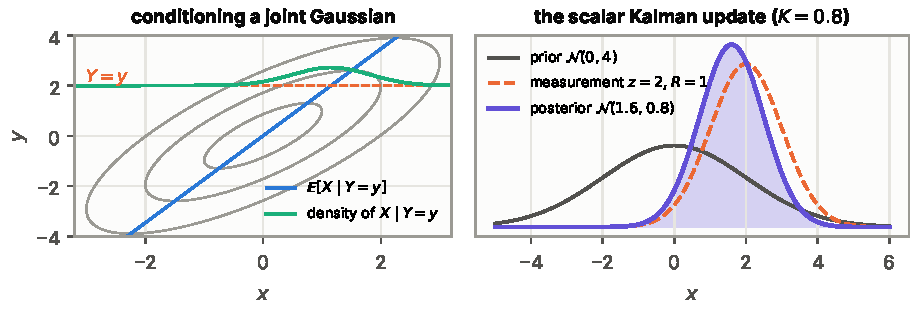
\includegraphics[width=\linewidth]{figures/ch03_gaussian.pdf}
\caption{Left: contours of a joint Gaussian of two scalars $(X,Y)$. Fixing $Y=y$
(dashed) slices it; the slice, divided by $p(y)$, is the Gaussian density
of $X\mid Y=y$, whose
mean lies on the regression line $\E[X\mid Y=y]$ and whose width does not
depend on $y$. Right: the Kalman update in one dimension, for a prediction
$\Normal(0,4)$ and a measurement $z=2$ with noise variance $R=1$
(\cref{ex:scalarkf}): the posterior is $\Normal(1.6,\,0.8)$, with the
gain $K=0.8$. The posterior lies between the prior and the measurement, closer
to the more precise one, and is narrower than both.}
\label{fig:gaussian}
\end{figure}

\section{The filter}

The Kalman filter applies to models in which the next state is a linear
function of the current state and of the control, and the measurement is a
linear function of the state, each with added Gaussian noise. The matrix
$F_t$ says how the state evolves by itself, $B_t$ how the control acts on
it, and $H_t$ which combination of the state the sensor sees.

\begin{definition}{Linear-Gaussian model}{lgmodel}
\begin{align*}
  \x_{t+1}&=F_t\x_t+B_t\uu_t+\w_t, & \w_t&\sim\Normal(\vect0,Q_t),\\
  \z_{t}&=H_t\x_t+\vv_t, & \vv_t&\sim\Normal(\vect0,R_t),
\end{align*}
with $\x_0\sim\Normal(\hx_0,P_0)$, $R_t\succ0$, and all noises
independent of each other and of $\x_0$.
\end{definition}

Two symbols are used throughout the book: a bar marks a \emph{predicted}
quantity (before the measurement), $\bx$ and $\bar P$; a hat marks an
\emph{updated} estimate (after it), $\hx$, with covariance $P$.

\paragraph{The update in one dimension.} The heart of the filter is
visible when the state is a single number $x$. Before the measurement,
the filter believes $x\sim\Normal(\bar x,\bar P)$. A sensor reads
$z=x+v$, with a noise $v\sim\Normal(0,R)$ independent of $x$. These are two
noisy pieces of information about the same number: the prediction
$\bar x$, of variance $\bar P$, and the reading $z$, of variance $R$. The pair $(x,z)$ is jointly Gaussian (\cref{lem:affine}), and, because
$x$ and $v$ are independent,
\[
  \Cov(x,z)=\Cov(x,x+v)=\Var(x)+\Cov(x,v)=\bar P+0,\qquad
  \Var(z)=\Var(x)+\Var(v)=\bar P+R .
\]
\Cref{thm:conditioning}, with $X=x$, $Y=z$, $\mu_x=\mu_y=\bar x$,
$\Sigma_{xy}=\bar P$ and $\Sigma_{yy}=\bar P+R$, gives the belief after the
measurement, $x\mid z\sim\Normal(\hat x,P)$, with the mean
$\bar x+\frac{\bar P}{\bar P+R}(z-\bar x)$ and the variance
$\bar P-\frac{\bar P^2}{\bar P+R}$. Naming the fraction $K$:
\begin{equation}\label{eq:scalarkf}
  \hat x=\bar x+K\,(z-\bar x),\qquad K=\frac{\bar P}{\bar P+R},\qquad
  P=(1-K)\,\bar P=\frac{\bar PR}{\bar P+R}.
\end{equation}
Three things can be read from these formulas.
\begin{itemize}[nosep]
  \item \emph{A weighted average.} $\hat x=(1-K)\,\bar x+K\,z$, with a
    weight $K$ between $0$ and $1$, the \emph{gain}. If the prediction is
    poor compared with the sensor ($\bar P\gg R$), $K$ is close to $1$ and
    the estimate follows the reading. If the sensor is poor, $K$ is close
    to $0$ and the reading is almost ignored.
  \item \emph{Precisions add.} The inverse of a variance is called a
    \emph{precision}, and
    $1/P=(\bar P+R)/(\bar PR)=1/R+1/\bar P$. The result is more precise
    than either source.
  \item \emph{The new variance does not depend on the reading.} $P$ is
    known before $z$ arrives.
\end{itemize}

\begin{example}{One update in one dimension}{scalarkf}
The prediction is $\Normal(0,4)$: the filter expects $x$ near $0$, give or
take $2$. The sensor has noise variance $R=1$ and reads $z=2$. Then $K=\bar P/(\bar P+R)=4/(4+1)=0.8$: the sensor is four times more
precise than the prediction, so the estimate moves four fifths of the way
towards the reading, $\hat x=\bar x+K(z-\bar x)=0+0.8\times(2-0)=1.6$. Its
variance is $P=(1-K)\bar P=(1-0.8)\times4=0.8$, smaller than both $4$ and
$1$; in precisions, $1/0.8=1.25=1/4+1/1$. This is the example drawn in \cref{fig:gaussian}, right.
\end{example}

The general filter is the same computation with matrices. It adds the
prediction step, and a matrix $H$ for sensors that measure a combination
of the coordinates of the state instead of the state itself.

\begin{theorem}{Kalman filter}{kf}
Under \cref{def:lgmodel}, every belief is Gaussian,
$\bel(\x_t)=\Normal(\hx_t,P_t)$, and $\belbar(\x_{t+1})=
\Normal(\bx_{t+1},\bar P_{t+1})$, with
\begin{align}
  &\textbf{predict:} & \bx_{t+1}&=F_t\hx_t+B_t\uu_t, &
  \bar P_{t+1}&=F_tP_tF_t\T+Q_t, \label{eq:kfpredict}\\
  &\textbf{update:} & \y&=\z_{t+1}-H\bx_{t+1}, & S&=H\bar P_{t+1}H\T+R,
  \notag\\
  && K&=\bar P_{t+1}H\T S^{-1}, & \hx_{t+1}&=\bx_{t+1}+K\y,\quad
  P_{t+1}=(I-KH)\bar P_{t+1}, \label{eq:kfupdate}
\end{align}
where $H$ and $R$ are taken at time $t+1$.
\end{theorem}

\begin{proof}
By induction on $t$. The belief $\bel(\x_0)=\Normal(\hx_0,P_0)$ is
Gaussian by assumption. Suppose that $\bel(\x_t)=\Normal(\hx_t,P_t)$.
Everything below is conditional on the past data (the controls and the
measurements up to time $t$); to lighten the notation, write $\x$, $\z$,
$\vv$, $\bx$ and $\bar P$ for $\x_{t+1}$, $\z_{t+1}$, $\vv_{t+1}$,
$\bx_{t+1}$ and $\bar P_{t+1}$.

\emph{Predict.} $\x_{t+1}=F_t\x_t+B_t\uu_t+\w_t$, where $\x_t\sim
\Normal(\hx_t,P_t)$, $B_t\uu_t$ is known, and $\w_t\sim\Normal(\vect0,
Q_t)$ is independent of $\x_t$ and of the past. \Cref{lem:affine}, with
$A=F_t$, $\vect b=B_t\uu_t$ and $W=\w_t$, gives
$\x_{t+1}\sim\Normal(F_t\hx_t+B_t\uu_t,\;F_tP_tF_t\T+Q_t)$: this is
\eqref{eq:kfpredict}.

\emph{The pair (state, measurement).} $\z=H\x+\vv$, with
$\vv\sim\Normal(\vect0,R)$ independent of $\x$. The pair $(\x,\z)$ is an
affine map of the independent Gaussians $\x$ and $\vv$, hence jointly
Gaussian (\cref{lem:affine}), with
\begin{align*}
  \bmu_y&=\E[H\x+\vv]=H\bx,\\
  \Sigma_{xy}&=\Cov(\x,H\x+\vv)=\Cov(\x,\x)H\T+\Cov(\x,\vv)
  =\bar PH\T+0,\\
  \Sigma_{yy}&=\Cov(H\x+\vv)=H\bar PH\T+R=S,
\end{align*}
the last line because the covariances of the independent $H\x$ and $\vv$
add.

\emph{Update.} \Cref{thm:conditioning}, with $X=\x$ and $Y=\z$, gives a
Gaussian with the mean and covariance
\begin{align*}
  \bx+\Sigma_{xy}\Sigma_{yy}^{-1}(\z-\bmu_y)
  &=\bx+\bar PH\T S^{-1}(\z-H\bx)=\bx+K\y,\\
  \bar P-\Sigma_{xy}\Sigma_{yy}^{-1}\Sigma_{yx}
  &=\bar P-\bar PH\T S^{-1}H\bar P=\bar P-KH\bar P=(I-KH)\bar P,
\end{align*}
using $\Sigma_{yx}=\Sigma_{xy}\T=H\bar P$ ($\bar P$ is symmetric). This
is \eqref{eq:kfupdate}, and $\bel(\x_{t+1})$ is Gaussian.
\end{proof}

The quantity $\y$ is the \emph{innovation}: what the measurement says that
the prediction did not. Its covariance is $S$ (Exercise~\ref{ex:innov}),
and $K$ is the \emph{Kalman gain}. In one dimension with $H=1$ these are
the formulas \eqref{eq:scalarkf}. The addition of precisions also holds in
any dimension.


\begin{proposition}{Information form}{information}
If $\bar P$ and $R$ are invertible, then
\[
  P^{-1}=\bar P^{-1}+H\T R^{-1}H\qquad\text{and}\qquad K=PH\T R^{-1}.
\]
\end{proposition}

\begin{proof}
To show that $P$ is the inverse of $\bar P^{-1}+H\T R^{-1}H$, multiply the
two and check that the product is $I$. Two identities are used:
$H\bar PH\T=S-R$, from the definition of $S$, and
\[
  S^{-1}(S-R)R^{-1}=S^{-1}SR^{-1}-S^{-1}RR^{-1}=R^{-1}-S^{-1} .
\]
Then, with $P=\bar P-\bar PH\T S^{-1}H\bar P$ from \cref{thm:kf}:
\begin{align*}
  P(\bar P^{-1}+H\T R^{-1}H)
  &=I+\bar PH\T R^{-1}H-\bar PH\T S^{-1}H
  &&\text{expand; }\bar P\bar P^{-1}=I\\
  &\qquad-\bar PH\T S^{-1}(H\bar PH\T)R^{-1}H\\
  &=I+\bar PH\T\bigl[R^{-1}-S^{-1}-S^{-1}(S-R)R^{-1}\bigr]H
  &&H\bar PH\T=S-R\\
  &=I+\bar PH\T\bigl[R^{-1}-S^{-1}-(R^{-1}-S^{-1})\bigr]H=I .
\end{align*}
For the gain:
\begin{align*}
  PH\T R^{-1}
  &=\bar PH\T R^{-1}-\bar PH\T S^{-1}(H\bar PH\T)R^{-1}
   =\bar PH\T R^{-1}-\bar PH\T S^{-1}(S-R)R^{-1}\\
  &=\bar PH\T R^{-1}-\bar PH\T(R^{-1}-S^{-1})=\bar PH\T S^{-1}=K .
\end{align*}
\end{proof}

\begin{inwords}
Information (inverse covariance) adds: what we knew, plus what the
measurement tells, and the measurement's contribution $H\T R^{-1}H$ does
not depend on what we knew. An update can only reduce the uncertainty, in every direction, as the
next paragraph shows. A direction $\vect n$ that the sensor
does not see ($H\vect n=\vect0$) receives no information from the
measurement itself: $\vect n\T P^{-1}\vect n=\vect n\T\bar P^{-1}\vect n$.
Its variance can still decrease, but only through its correlation with the
directions that the sensor does see; this is how a position fix can
correct a heading.
\end{inwords}

\emph{Why an update never increases a variance.} The variance of the
error along a direction $\vect n$ is $\vect n\T P\vect n$. With
$P=\bar P-\bar PH\T S^{-1}H\bar P$,
\[
  \vect n\T P\vect n=\vect n\T\bar P\vect n-\vect m\T S^{-1}\vect m,
  \qquad\vect m=H\bar P\vect n,
\]
because $\vect n\T\bar PH\T=(H\bar P\vect n)\T=\vect m\T$, $\bar P$ being
symmetric. $S^{-1}$ is positive definite (the inverse of the positive
definite $S$), so $\vect m\T S^{-1}\vect m\ge0$ and
$\vect n\T P\vect n\le\vect n\T\bar P\vect n$.

\begin{proposition}{Joseph form}{joseph}
Let the prediction error $\x-\bx$ have mean zero and covariance $\bar P$
and be independent of the measurement noise $\vv$. For \emph{any} gain
$K$, the error of the estimate $\hx=\bx+K(\z-H\bx)$ has covariance
\begin{equation}\label{eq:joseph}
  P_K=(I-KH)\bar P(I-KH)\T+KRK\T,
\end{equation}
which is positive semi-definite. For the Kalman gain it equals
$(I-KH)\bar P$.
\end{proposition}

\begin{proof}
\emph{The error.} With $\z=H\x+\vv$,
\[
  \x-\hx=\x-\bx-K(H\x+\vv-H\bx)=(I-KH)(\x-\bx)-K\vv ,
\]
a sum of two independent zero-mean terms, with the covariances
$(I-KH)\bar P(I-KH)\T$ and $K RK\T$ (by $\Cov(AX)=A\Cov(X)A\T$). The
covariances of independent terms add, which gives \eqref{eq:joseph}: a
sum of two positive semi-definite matrices, hence positive
semi-definite.

\emph{The Kalman gain.} Expand the product:
\begin{align*}
  P_K&=\bar P-KH\bar P-\bar PH\T K\T+KH\bar PH\T K\T+KRK\T\\
  &=\bar P-KH\bar P-\bar PH\T K\T+KSK\T
  &&H\bar PH\T+R=S .
\end{align*}
With $K=\bar PH\T S^{-1}$, the last term is $KSK\T=\bar PH\T S^{-1}SK\T=
\bar PH\T K\T$, which cancels the third, and $P_K=\bar P-KH\bar P=(I-KH)
\bar P$.
\end{proof}

The short form $(I-KH)\bar P$ is the difference of two positive
semi-definite matrices; rounding errors can make it slightly asymmetric
or indefinite, and the next update may then fail. The Joseph form is a sum
of positive semi-definite terms and does not have that problem, which is
why the code uses it. It also gives the true error covariance when the
gain is wrong, for instance because the filter was given the wrong $R$
(Exercise~\ref{ex:wrongR}).

\section{A linear robot}
\label{sec:linmower}

The pose model of Chapter~\ref{ch:statespace} is not linear: the heading
enters through $\cos$ and $\sin$. We make it linear honestly, with the
compass. The robot drives from $\p_t$ to $\p_{t+1}$ along the heading
$\theta_{t+1}$ that it has after its turn. Let
$c_{t+1}=\wrap(\theta_{t+1}+\nu_{t+1})$ be the compass reading of that
heading (\cref{sec:sensors}). With the heading read off the compass, the
displacement is a \emph{known input}. The turn error $\varepsilon_\delta$
no longer matters: whatever heading the robot ends up with, the compass
reads it. The position obeys
\begin{equation}\label{eq:linmower}
  \p_{t+1}=\p_t+s_t\begin{pmatrix}\cos c_{t+1}\\\sin c_{t+1}\end{pmatrix}
  +\w_t,\qquad\z_{t+1}=\p_{t+1}+\vv_{t+1},
\end{equation}
so $F=B=H=I$ and $R=\sigma_{\mathrm{gps}}^2I=64\,I$
($\sigma_{\mathrm{gps}}=8$). The noise $\w_t$ is the difference between
the true displacement and the one computed from the compass. The true
displacement is $(s_t+\varepsilon_s)(\cos\theta_{t+1},\sin\theta_{t+1})$
with $\theta_{t+1}=c_{t+1}-\nu_{t+1}$. To first order in the small angle
$\nu=\nu_{t+1}$, writing $c=c_{t+1}$,
\[
  \cos(c-\nu)\approx\cos c+\nu\sin c,\qquad
  \sin(c-\nu)\approx\sin c-\nu\cos c ,
\]
and, dropping the product $\varepsilon_s\nu$ of two small noises,
\[
  (s_t+\varepsilon_s)\begin{pmatrix}\cos(c-\nu)\\\sin(c-\nu)\end{pmatrix}
  \approx s_t\begin{pmatrix}\cos c\\\sin c\end{pmatrix}
  +\varepsilon_s\begin{pmatrix}\cos c\\\sin c\end{pmatrix}
  +(-\nu)\,s_t\begin{pmatrix}-\sin c\\\cos c\end{pmatrix}.
\]
The first term is the computed displacement, and the other two are the
noise:
\[
  \w_t\approx G_t\begin{pmatrix}\varepsilon_s\\-\nu_{t+1}\end{pmatrix},\quad
  G_t=\begin{pmatrix}\cos c_{t+1}&-s_t\sin c_{t+1}\\
  \sin c_{t+1}&s_t\cos c_{t+1}\end{pmatrix},\qquad
  Q_t=G_t\diag(\sigma_s^2,\sigma_c^2)\,G_t\T ,
\]
the covariance following from $\Cov(AX)=A\Cov(X)A\T$, with
$\Cov(\varepsilon_s,-\nu_{t+1})=\diag(\sigma_s^2,\sigma_c^2)$ for
independent noises.
This is the computation of \cref{sec:errors} again: an error on the
distance moves the robot along its heading, and an error on the heading,
here the compass error, moves it sideways by $s_t$ per radian. $G_t$ is the upper $2\times2$ block of the matrix
$V=\bigl(\begin{smallmatrix}\cos\theta'&-s\sin\theta'\\\sin\theta'&s\cos\theta'\\0&1\end{smallmatrix}\bigr)$
of \eqref{eq:firstorder}, whose columns give the effects on the pose of a
distance error and of a heading error, with the heading $\theta'$ replaced
by the compass reading $c_{t+1}$.
One more approximation is made, beyond the first order: the compass noise
$\nu_{t+1}$ enters both the known input $c_{t+1}$ and the noise $\w_t$, so
$\w_t$ is not exactly independent of the input. The effect is small
($\sigma_c=0.02$\,rad), and the consistency test of \cref{fig:kfnees}
shows that the filter is not misled by it.
$Q_t$ is long along the heading (step noise) and thin across it (compass
noise), and it turns with the robot. A time-varying $Q_t$ is no problem:
nothing in \cref{thm:kf} needs it to be constant.

\Cref{fig:kftrack} shows the filter on the standard run. Once it has
settled (after the first 20 steps), its RMS position error is $1.99$,
against $11.3$ for the raw GPS fixes (notebook~02): filtering divides the
error by $11.3/1.99\approx5.7$.

\begin{figure}[ht]
\centering
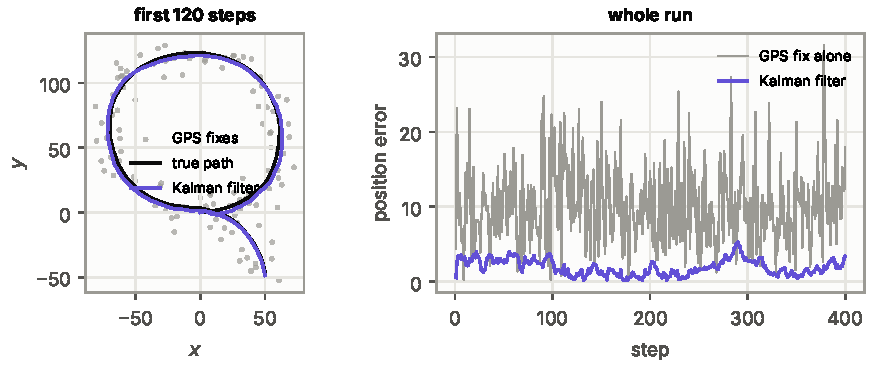
\includegraphics[width=\linewidth]{figures/ch03_kf_track.pdf}
\caption{The Kalman filter of the linear robot, which takes its heading
from the compass and corrects its position with GPS fixes
($\sigma_{\mathrm{gps}}=8$), on the standard run (seed 1). Left: the true
path, the GPS fixes and the filter's estimate over the first 120 steps.
Right: the position error of each GPS fix and of the filter over the
whole run.}
\label{fig:kftrack}
\end{figure}

\section{The gain settles}

When $F$, $H$, $Q$ and $R$ are fixed in advance, $P_t$ and $K_t$ do not
depend on the measurements: only on these matrices and on $P_0$. (In the
compass--GPS filter they depend on the compass readings, through $Q_t$,
but not on the GPS fixes.) For a time-invariant model the predicted covariance obeys the
\emph{Riccati recursion} $\bar P\mapsto F\bigl(\bar P-\bar PH\T(H\bar PH\T
+R)^{-1}H\bar P\bigr)F\T+Q$, which converges, under mild conditions, to a
unique fixed point. (The conditions are called detectability and
stabilisability. Roughly: the sensor sees every direction of the state in
which the error would otherwise grow, and the noise $Q$ excites every such
direction. The general result is not proved here; see Bar-Shalom, Li and
Kirubarajan in the references.) The scalar case can be solved by hand, and
\cref{fig:riccati} shows the convergence.

\begin{proposition}{Steady state of a random walk observed in noise}{steady}
For the scalar model $x_{t+1}=x_t+w_t$, $z_t=x_t+v_t$ with variances $q>0$
and $r>0$, the steady-state predicted and updated variances are
\[
  \bar P_\infty=\frac{q+\sqrt{q^2+4qr}}2,\qquad
  P_\infty=\frac{\bar P_\infty r}{\bar P_\infty+r}=\bar P_\infty-q .
\]
\end{proposition}

\begin{proof}
\emph{The fixed point.} With $F=H=1$, the update gives
$P=\bar Pr/(\bar P+r)$ (\cref{eq:scalarkf}) and the next prediction gives
$\bar P=P+q$. At a fixed point both hold with the same $\bar P$:
\begin{align*}
  \bar P&=\frac{\bar Pr}{\bar P+r}+q\\
  \bar P(\bar P+r)&=\bar Pr+q(\bar P+r)
  &&\text{multiply by }\bar P+r\\
  \bar P^2-q\bar P-qr&=0
  &&\text{expand; }\bar Pr\text{ cancels.}
\end{align*}
This quadratic has the roots $\bigl(q\pm\sqrt{q^2+4qr}\bigr)/2$; one is
negative, and the positive one is $\bar P_\infty$. Then
$P_\infty=\bar P_\infty-q$ from $\bar P=P+q$.

\emph{Convergence.} One cycle maps $\bar P$ to
$g(\bar P)=\bar Pr/(\bar P+r)+q$, whose derivative is
\[
  g'(\bar P)=\frac{r(\bar P+r)-\bar Pr}{(\bar P+r)^2}
  =\frac{r^2}{(\bar P+r)^2}.
\]
After the first cycle $\bar P\ge q$, since $g(\bar P)\ge q$. On
$[q,\infty)$, $0<g'\le c$ with $c=r^2/(q+r)^2<1$. By the mean value
theorem, $\abs{g(a)-g(b)}=g'(\xi)\abs{a-b}\le c\,\abs{a-b}$ for $a,b$ in
that interval. With $b=\bar P_\infty$, a fixed point, the distance to
$\bar P_\infty$ is multiplied by at most $c$ at each cycle, so after $t$
more cycles it is at most $c^t$ times the initial distance, which tends to
$0$: the recursion converges to $\bar P_\infty$ from any start.
\end{proof}

\begin{figure}[ht]
\centering
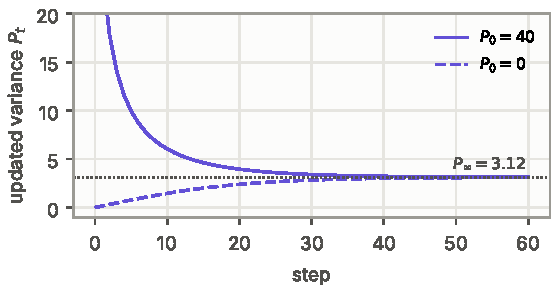
\includegraphics{figures/ch03_riccati.pdf}
\caption{The updated variance $P_t$ of the scalar model
$x_{t+1}=x_t+w_t$, $z_t=x_t+v_t$, with $q=0.16$ and $r=64$ (the values of
the robot along its heading), from an uncertain start $P_0=40$ (solid) and
from an exactly known start $P_0=0$ (dashed). Both converge to the same $P_\infty$: the filter forgets
its initial uncertainty.}
\label{fig:riccati}
\end{figure}

For the robot, $r=\sigma_{\mathrm{gps}}^2=64$ in both directions. Along
the heading, $q=\sigma_s^2=0.4^2=0.16$, and
\[
  \bar P_\infty=\frac{0.16+\sqrt{0.16^2+4\times0.16\times64}}{2}
  =\frac{0.16+6.402}{2}=3.28,\qquad P_\infty=3.28-0.16=3.12 .
\]
Across it, $q=(s\sigma_c)^2=(4\times0.02)^2=0.0064$, and the same formulas
give $\bar P_\infty=(0.0064+1.280)/2=0.643$ and $P_\infty=0.64$. If the heading
were constant, the RMS error would therefore settle at
$\sqrt{3.12+0.64}=1.94$. Because the heading turns, the long axis of $Q_t$
rotates and the two directions mix. Averaged over the headings, $Q_t$ is
about $\tfrac12(0.16+0.0064)\,I=0.0832\,I$: with $q_1=0.16$ along the
heading $c$ and $q_2=0.0064$ across it, the entries of $Q_t$ are
$q_1\cos^2c+q_2\sin^2c$, $q_1\sin^2c+q_2\cos^2c$ on the diagonal and
$(q_1-q_2)\sin c\cos c$ off it, and over a full turn $\cos^2$ and
$\sin^2$ average to $\tfrac12$ and $\sin c\cos c$ to $0$. Then \cref{prop:steady} with $q=0.0832$ gives
$\bar P_\infty=(0.0832+\sqrt{0.0832^2+4\times0.0832\times64})/2=2.35$ and
$P_\infty=2.35-0.08=2.27$ per axis, a trace of $2\times2.27=4.5$. The filter's
own covariance indeed settles around $\operatorname{tr}P\approx4.5$, i.e.\
an RMS of $2.1$, and the measured RMS error over 20 runs (seeds 0 to 19,
started at the true pose with $P_0=\diag(400,400)$, the first 20 steps
left out) is $2.11$ (notebook~02). The filter's covariance is
telling the truth, which is the subject of the next section.

\section{Is the filter honest? NEES}

A small error is not enough: the filter must also \emph{know} how large
its error is, because its covariance is what the next update, and every
decision downstream, relies on.

\begin{definition}{NEES}{nees}
The \emph{normalised estimation error squared} at time $t$ is
\[
  \NEES_t=(\x_t-\hx_t)\T P_t^{-1}(\x_t-\hx_t).
\]
\end{definition}

The NEES is the squared error measured in units of the covariance the
filter claims: in one dimension it is $(x-\hat x)^2/P$, which is $1$ on
average when the claim is right. An error of $3$ with a claimed standard
deviation of $1$ gives a NEES of $9$: a ``three-sigma'' error, which
should be rare. Recall that $\chi^2_n$ (chi-squared with
$n$ degrees of freedom) is the distribution of the sum of the squares of
$n$ independent standard normal variables; its mean is $n$.

For the Kalman filter of a linear-Gaussian model, the hypothesis of the
next proposition is the conclusion of \cref{thm:kf}: given the data, the
error $\x_t-\hx_t$ is $\Normal(\vect0,P_t)$.

\begin{proposition}{NEES of a consistent filter}{neeschi2}
If $\x_t-\hx_t\sim\Normal(\vect0,P_t)$ with $P_t\succ0$ in $\R^n$, then
$\NEES_t\sim\chi^2_n$, so $\E[\NEES_t]=n$. If $\NEES^{(1)},\dots,
\NEES^{(N)}$ are the values from $N$ independent runs, then
$N\cdot\frac1N\sum_k\NEES^{(k)}\sim\chi^2_{nN}$.
\end{proposition}

\begin{proof}
Let $L$ with $LL\T=P_t$ (Cholesky), and $\vect g=L^{-1}(\x_t-\hx_t)$. By
\cref{lem:affine}, $\vect g$ is Gaussian with mean $\vect0$ and
covariance $L^{-1}P_tL^{-\mathsf T}=L^{-1}LL\T L^{-\mathsf T}=I$, so its
coordinates are independent standard normals (\cref{lem:uncorr}). Then
\[
  \NEES_t=(\x_t-\hx_t)\T(LL\T)^{-1}(\x_t-\hx_t)
  =\bigl(L^{-1}(\x_t-\hx_t)\bigr)\T L^{-1}(\x_t-\hx_t)
  =\vect g\T\vect g=\sum_{i=1}^ng_i^2 ,
\]
a sum of $n$ squared independent standard normals: $\chi^2_n$, of mean
$n$, since each square has the mean $\E[g_i^2]=\Var(g_i)=1$. The $N$ runs are independent, so the sum
of their NEES is a sum of $nN$ squares of independent standard normals,
that is $\chi^2_{nN}$.
\end{proof}

A two-sided $95\%$ acceptance band for the average NEES over $N$ runs is
therefore
\[
  \bigl[\chi^2_{nN}(0.025),\;\chi^2_{nN}(0.975)\bigr]\big/N,
\]
where $\chi^2_k(p)$ is the $p$-quantile of $\chi^2_k$: the value below
which $\chi^2_k$ falls with probability $p$. For example, with $n=2$
and $N=50$ runs, $\chi^2_{100}(0.025)=74.2$ and
$\chi^2_{100}(0.975)=129.6$, and the band is $[1.48,\,2.59]$
(notebook~02). Above it, the
filter is \emph{over-confident}: it claims more precision than it has.
Below it, it is \emph{pessimistic}. For the test to be fair, the initial
estimate must itself be drawn from the initial belief,
$\hx_0\sim\Normal(\x_0,P_0)$; starting exactly at the truth with a large
$P_0$ would make the first steps look pessimistic.

\begin{figure}[ht]
\centering
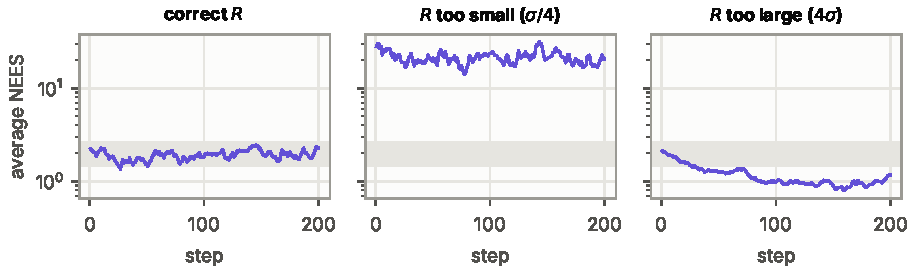
\includegraphics[width=\linewidth]{figures/ch03_kf_nees.pdf}
\caption{Average NEES over 50 runs (log scale) for the Kalman filter of
the linear robot (compass heading, GPS fixes with
$\sigma_{\mathrm{gps}}=8$); grey: the $95\%$ band for $n=2$,
$[1.48,\,2.59]$. Left: the correct $R$,
inside the band. Middle: the filter believes that the standard deviation
of the GPS is 4 times smaller than it is ($R/16$): over-confident by an
order of magnitude. Right: it believes it is 4 times larger ($16R$):
pessimistic.}
\label{fig:kfnees}
\end{figure}

\begin{inwords}
NEES asks: ``are the errors as big as the filter says they are?'' A
filter that believes its sensor too much is jumpy \emph{and} certain; one
that believes it too little is sluggish and doubtful. NEES needs the
truth, so it is a simulation tool. On real data the same idea is applied
to the innovations: for a correct filter the innovation is
$\Normal(\vect0,S)$ (Exercise~\ref{ex:innov}), so
$\y\T S^{-1}\y\sim\chi^2_{\dim\z}$ by the same argument (the \emph{NIS}
test), and that one only needs the data.
\end{inwords}

\begin{practice}[\nb{02\_kalman\_filter.ipynb}, \code{kf.py}, \code{metrics.py}]
\code{KalmanFilter} is the generic filter of \cref{thm:kf}, with the
Joseph update; \code{CompassGpsKF} builds $Q_t$ from the compass reading
at each step. \code{nees} and \code{nees\_bounds} implement
\cref{def:nees} and the $\chi^2$ band. The notebook checks the scalar
example $\Normal(0,4)$ updated by a measurement $2$ of variance $1$
(posterior $\Normal(8/5,4/5)$, gain $0.8$), shows the gain settling, and
reproduces \cref{fig:kfnees}.
\end{practice}

\begin{mower}
Wheel odometry plus RTK-GNSS is exactly this filter, and a common design
for robot mowers. RTK fixes are accurate to about 2\,cm with an open sky,
but degrade near trees and walls, sometimes without warning. A filter
with a fixed, optimistic $R$ is then the middle panel of
\cref{fig:kfnees}: it follows a bad fix with full confidence. Monitoring
the NIS and inflating $R$ (or rejecting the fix) when it leaves its band
is a cheap and effective guard.
\end{mower}

\section*{What to remember from this chapter}
\addcontentsline{toc}{section}{What to remember}

\begin{enumerate}[nosep]
  \item For a linear model with Gaussian noises, the belief is exactly
    Gaussian, and the Bayes filter reduces to formulas on its mean and
    covariance: the Kalman filter (\cref{thm:kf}).
  \item Predict: the mean follows the model and the covariance grows,
    $\bar P=FPF\T+Q$. Update: the mean moves by gain times innovation,
    $\hx=\bx+K\y$, and the covariance shrinks.
  \item The gain weighs the prediction against the measurement according
    to their precisions. In information form, precisions add:
    $P^{-1}=\bar P^{-1}+H\T R^{-1}H$.
  \item The covariance and the gain do not depend on the measurements, and
    for a time-invariant model they settle to constants.
  \item A filter is \emph{consistent} when its errors are as large as its
    covariance says. The NEES test checks this in simulation, the NIS test
    on real data. A wrong $R$ or $Q$ makes the filter over-confident or
    pessimistic.
\end{enumerate}

\FloatBarrier
\section*{Exercises}
\addcontentsline{toc}{section}{Exercises}

\begin{enumerate}[label=\textbf{3.\arabic*},ref=3.\arabic*]
\item\label{ex:innov} Show that, for the Kalman filter, the innovation
  $\y=\z-H\bx$ has mean zero and covariance $S$, and that it is
  uncorrelated with the error of the estimate \emph{after} the update,
  i.e.\ $\Cov(\x-\hx,\y)=0$.
\item\label{ex:fusion} Two independent sensors measure the same scalar,
  with variances $r_1$ and $r_2$, and there is no prior ($\bar P=\infty$).
  Using \cref{prop:information} (precisions add,
$P^{-1}=\bar P^{-1}+H\T R^{-1}H$, and $K=PH\T R^{-1}$), show that the
optimal estimate is the
  inverse-variance weighted average and give its variance. What happens
  when $r_2\to\infty$?
\item\label{ex:steadynum} Use \cref{prop:steady} to compute the
  steady-state gain $K_\infty=\bar P_\infty/(\bar P_\infty+r)$ along the
  heading for the robot ($q=0.16$, $r=64$). How many past GPS fixes does
  the filter effectively average?
\item\label{ex:wrongR} A Kalman filter is run with a wrong measurement
  covariance $R'$ while the true one is $R$. Show that the covariance it
  reports follows the Riccati recursion with $R'$, while the covariance of
  its actual error follows a linear recursion that uses the filter's gain
  and the true $R$; write that recursion. Explain the middle panel of
  \cref{fig:kfnees}.
\end{enumerate}

\subsection*{Solutions}

\solution{3.1} Everything is conditional on the past data, and the
prediction error $\x-\bx$ has mean $\vect0$ and covariance $\bar P$
(\cref{thm:kf}).

\emph{Mean and covariance of the innovation.} With $\z=H\x+\vv$,
\[
  \y=\z-H\bx=H(\x-\bx)+\vv .
\]
Both terms have mean zero, so $\E[\y]=\vect0$. They are independent (the
noise $\vv$ is independent of the state and of the past), so their
covariances add:
$\Cov(\y)=H\,\Cov(\x-\bx)\,H\T+\Cov(\vv)=H\bar PH\T+R=S$.

\emph{The updated error and the innovation.} After the update,
$\x-\hx=\x-\bx-K\y$. The cross-covariance is linear in each argument, so
\[
  \Cov(\x-\hx,\y)=\Cov(\x-\bx,\y)-K\Cov(\y,\y)=\Cov(\x-\bx,\y)-KS .
\]
The first term is
$\Cov(\x-\bx,\,H(\x-\bx)+\vv)=\Cov(\x-\bx,\x-\bx)H\T+\Cov(\x-\bx,\vv)
=\bar PH\T+0$, and for the Kalman gain $KS=\bar PH\T S^{-1}S=\bar PH\T$.
So
\[
  \Cov(\x-\hx,\y)=\bar PH\T-\bar PH\T=0 .
\]
The updated error is uncorrelated with the innovation, and, the two being
jointly Gaussian, independent of it (\cref{lem:uncorr}): the filter has
extracted everything the measurement had to say.

\solution{3.2} \emph{The estimate in information form.} By
\cref{prop:information}, $P^{-1}=\bar P^{-1}+H\T R^{-1}H$ and
$K=PH\T R^{-1}$. The update can be written
$\hx=\bx+K(\z-H\bx)=(I-KH)\bx+K\z$, and
\[
  I-KH=I-PH\T R^{-1}H=P\bigl(P^{-1}-H\T R^{-1}H\bigr)=P\bar P^{-1},
\]
so
\[
  \hx=P\bigl(\bar P^{-1}\bx+H\T R^{-1}\z\bigr),\qquad
  P^{-1}=\bar P^{-1}+H\T R^{-1}H .
\]

\emph{No prior.} ``No prior'' is the limit $\bar P\to\infty$, where the
prior precision $\bar P^{-1}$ tends to $0$. Then
$P^{-1}=H\T R^{-1}H$ and $\hx=PH\T R^{-1}\z$.

\emph{Two sensors.} Stack the two readings into $\z=(z_1,z_2)$: both
measure the same scalar $x$, so $H=(1,1)\T$, and the noises are
independent, so $R=\diag(r_1,r_2)$. Then
\[
  H\T R^{-1}H=\frac1{r_1}+\frac1{r_2},\qquad
  H\T R^{-1}\z=\frac{z_1}{r_1}+\frac{z_2}{r_2},
\]
and
\[
  \hat x=\frac{z_1/r_1+z_2/r_2}{1/r_1+1/r_2}
  =\frac{r_2z_1+r_1z_2}{r_1+r_2},\qquad
  P=\frac{1}{1/r_1+1/r_2}=\frac{r_1r_2}{r_1+r_2}.
\]
This is the average of the readings weighted by their precisions $1/r_1$
and $1/r_2$, and its variance is smaller than both $r_1$ and $r_2$.

\emph{A useless second sensor.} When $r_2\to\infty$, the weight
$1/r_2$ tends to $0$: $\hat x\to z_1$ and $P\to r_1$. A sensor that tells
nothing is ignored; it never makes the estimate worse.

\solution{3.3} The robot along its heading is the model of
\cref{prop:steady} with $q=\sigma_s^2=0.16$ and $r=\sigma_{\mathrm{gps}}^2
=64$. The steady state is
\begin{align*}
  \bar P_\infty&=\frac{q+\sqrt{q^2+4qr}}{2}
  =\frac{0.16+\sqrt{0.0256+40.96}}{2}=3.28,\\
  K_\infty&=\frac{\bar P_\infty}{\bar P_\infty+r}=\frac{3.28}{3.28+64}
  =0.049 .
\end{align*}

\emph{An exponential moving average.} In steady state the update is
$\hat x_t=\bar x_t+K(z_t-\bar x_t)=(1-K)\bar x_t+Kz_t$, and the prediction
$\bar x_t=\hat x_{t-1}+d_{t-1}$ adds the known displacement. Leaving the
displacements aside, unrolling the recursion gives
\[
  \hat x_t=Kz_t+K(1-K)z_{t-1}+K(1-K)^2z_{t-2}+\cdots :
\]
the fix of $k$ steps ago has the weight $K(1-K)^k$, and the weights add up
to $K\sum_k(1-K)^k=K/K=1$. This is an \emph{exponential moving average},
a causal one: only past fixes enter.

\emph{How many fixes.} The weights decay by the factor $1-K$ per step;
their effective number is about $1/K=1/0.049\approx20$. The variance gives
the same count: an average of $m$ independent fixes has the variance
$r/m=64/m$, which equals $P_\infty=\bar P_\infty-q=3.12$ for
$m=64/3.12\approx20.5$.

\solution{3.4} \emph{What the filter reports.} The filter computes its
covariances and gains from its own recursion, as if the measurement
covariance were $R'$:
\[
  \bar P'\mapsto F\bigl(\bar P'-\bar P'H\T(H\bar P'H\T+R')^{-1}H\bar
  P'\bigr)F\T+Q,\qquad K'=\bar P'H\T(H\bar P'H\T+R')^{-1}.
\]
This is the Riccati recursion with $R'$, and $\bar P'$ is what it
reports.

\emph{What its error really is.} Its actual error obeys
$\x-\hx=(I-K'H)(\x-\bx)-K'\vv$, with the true noise
$\vv\sim\Normal(\vect0,R)$. \Cref{prop:joseph} holds for any gain, so the
actual covariance follows the linear recursion
\[
  P^{\mathrm{true}}=(I-K'H)\,\bar P^{\mathrm{true}}(I-K'H)\T+K'R{K'}\T,
  \qquad\bar P^{\mathrm{true}}\leftarrow FP^{\mathrm{true}}F\T+Q ,
\]
with the filter's gain $K'$ and the true $R$.

\emph{The middle panel of \cref{fig:kfnees}.} The filter believes
$R'=R/16$. Take the scalar values of \cref{prop:steady}: $F=H=1$,
$q=0.16$, the true $r=64$ and the believed $r'=64/16=4$. The filter's own
steady state is
\[
  \bar P'_\infty=\frac{0.16+\sqrt{0.16^2+4\times0.16\times4}}{2}=0.88,
  \qquad K'=\frac{0.88}{0.88+4}=0.181,
\]
against $0.049$ with the right $r$: the filter averages fewer fixes. The
variance it reports is $P'_\infty=\bar P'_\infty-q=0.88-0.16=0.72$. The
actual variance $P$ is the fixed point of the recursion above:
\begin{align*}
  P&=(1-K')^2(P+q)+K'^2r
  &&\text{fixed point}\\
  P\bigl(1-(1-K')^2\bigr)&=(1-K')^2q+K'^2r
  &&\text{collect }P\\
  P&=\frac{0.819^2\times0.16+0.181^2\times64}{1-0.819^2}
  =\frac{0.107+2.10}{0.329}\approx6.7
  &&K'=0.181,
\end{align*}
about nine times the reported $0.72$. NEES measures the actual error in
units of the reported covariance, hence values an order of magnitude
above the band.
